\begin{figure}[h!]
    \centering
    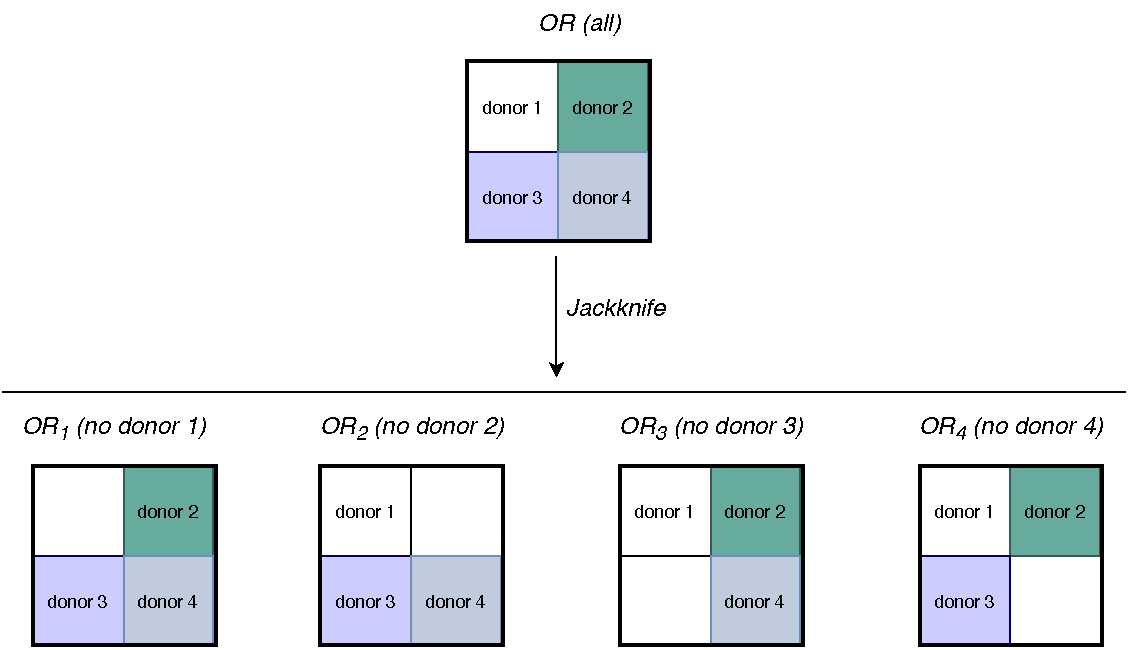
\includegraphics[scale=0.8]{graphics/jackknife_demo.pdf}
    \caption{\textbf{Illustration of jackknife analysis}. For a hypothetical cancer with 4 donors, the original odds ratio $OR$ was computed. Donor 1 was then omitted and a new odds ratio $OR_1$ was recomputed and a pseudo value $OR^{pseudo}_1$ was obtained. The same was applied to every other donor. The end result was a set of odds ratio statistics $\{OR_1^{pseudo}, \ldots, OR_4^{pseudo}\}$ that were used to estimate the possible range of the true $OR$ statistic}
    \label{fig:jackknife_demo}
\end{figure}
